\section{Comptonův jev}
    \subsection{Comptonův rozptyl}
        Odvoďte vztah pro energii fotonu $E'_{\gamma}$ a jeho vlnovou délku $\lambda'$, který se rozptýlil na elektronu na úhel $\theta$ (obrázek~\ref{fig:Compton}).
        Energie a vlnová délka fotonu před rozptylem je $E_{\gamma}$ a $\lambda$.
        Předpokládejte, že před rozptylem je elektron v klidu.
        Hmotnost elektronu je $m_{e}$.

        \begin{figure}[!h]
            \centering
            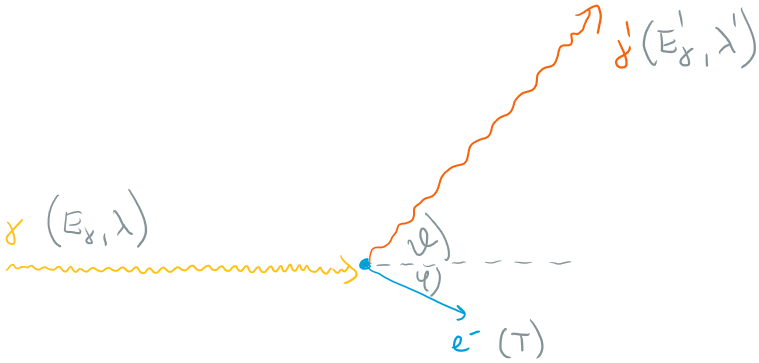
\includegraphics[width=0.6\linewidth]{Compton.png}
            \caption{Comptonův rozptyl fotonu $\gamma$ na elektronu $e^{-}$.}
            \label{fig:Compton}
        \end{figure}

    \subsection{Comptonova vlnová délka}
        Vyjádřete vztah pro změnu vlnové délky fotonu při Comptonově rozptylu $\Delta\lambda=\lambda'-\lambda$ pomocí Comptonovy vlnové délky $\lambda_{c}=h/(m_{e}c)$, kde $h$ je Planckova konstanta, $m_{e}$ hmotnost elektronu a $c$ rychlost světla.

    \subsection{Úhel vylétávajícího elektronu}
        Odvoďte vztah pro úhel $\varphi$, pod kterým vylétá elektron po Comptonově rozptylu (obrázek~\ref{fig:Compton}).

    \subsection{Spektrum $\gamma$ při měření v detektoru}
        \begin{figure}[!h]
            \centering
            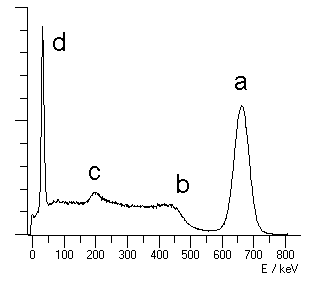
\includegraphics[width=0.35\linewidth]{ComptonSpectrum.png}
            \caption{Detekované Comptonovské spektrum monochromatického $\gamma$ záření.}
            \label{fig:ComptonSpectrum}
        \end{figure}        
    
        Detektor vysokoenergetických kvant $\gamma$ funguje na principu Comptonova rozptylu, kdy kinetická energie rozptýlených elektronů vytvoří impuls elektrického proudu, který se následně zesílí a změří.

        Předpokládejte, že na detektor dopadá monochromatické záření s energií kvant $E_{\gamma}$ vzniklé rozpadem radioaktivního nuklidu.
        Vysvětlete body a, b, c z obrázku~\ref{fig:ComptonSpectrum}; obrázek zobrazuje četnost, se kterou byla detektorem naměřena energie elektronu $E$. 
        Odhadněte, jaká byla energie $E_{\gamma}$, a z této \href{https://cds.cern.ch/record/1309915/files/978-3-642-02586-0_BookBackMatter.pdf}{tabulky} určete nuklid, jehož rozpad je měřen.

        % Zdroj tabulky: https://www.ld-didactic.de/software/524221en/Content/Appendix/ComptonSpectrum.htm